\section{Silicon Vertex Tracker (SVT)}

Ο Silicon Vertex Tracker (SVT) είναι ένα σύστημα που βασίζεται σε τρία στώματα από Silicon Drift Detectors (SDDs) και μπορεί να δώσει διδιάστατες ανιχνεύσεις με ανιχνευτική ικανότητα της τάξης των 20μm σε κάθε διέυθυνση. Ακόμη, συνεισφέρει στην ταυτοποίηση των σωματιδίων καθώς παρέχει επίσης καλή διακριτική ικανότητα στις μετρήσεις απωλειών ενέργειας. 
	Πέρα από αυτές τις συνεισφορές, οι οποίες βελτιώνουν διαδικασίες που πραγματοποιούνται και από άλλα όργανα του STAR, ο SVT προσδίδει μία επιπλέον δυνατότητα ανίχνευσης που δεν προσφέρουν οι υπόλοιποι ανιχνευτές.
	Δεδομένου ότι είναι ο πιο κοντινός ανιχνευτής στην δέσμη (Εικόνα \ref{fig3.2}), μπορεί να ανακατασκευάζει τροχιές από σωματίδια με πολύ μικρό χρόνο ζωής, όπως  D-μεσόνια και strange \& mulitystrange βαρυόνια τα οποία αναμένεται να υπάρχουν σε αφθονία στο Quark Gluon Plasma.
	Ακόμη, επεκτείνει την αποδοχή του ανιχνευτή και σε σωματίδια με πολύ χαμηλή ορμή τα οποία λόγω του μαγνητικού πεδίου δεν προλαβαίνουν να φτάσουν στον TPC.


%%%%%%%%%%%%%%%%%%%%%%%%%%55
%%% na valw to label
%	\begin{figure}[h!]
%		\centering 
%		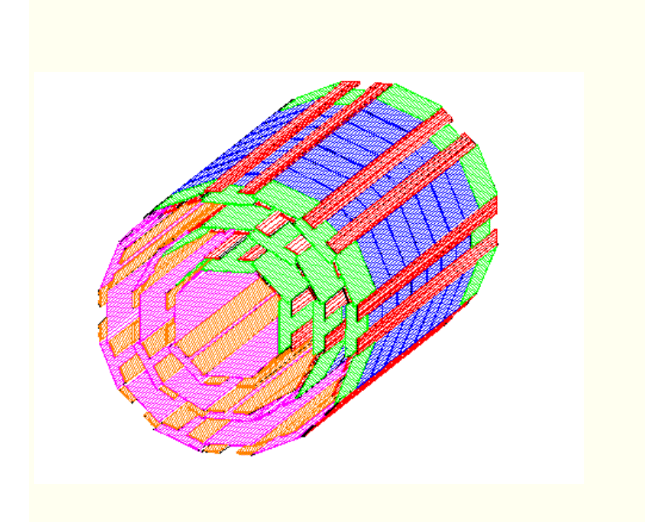
\includegraphics[scale=0.5]{STAR_Detectors/SVD_3_Layers}
%		\caption{Τα τρία στρώματα από SDD του SVT}
%		\label{fig3.13}
%	\end{figure}
	
	\begin{figure}[h!]
    \centering
    \subfloat[\centering Τα τρία στρώματα από SDD του SVT]{{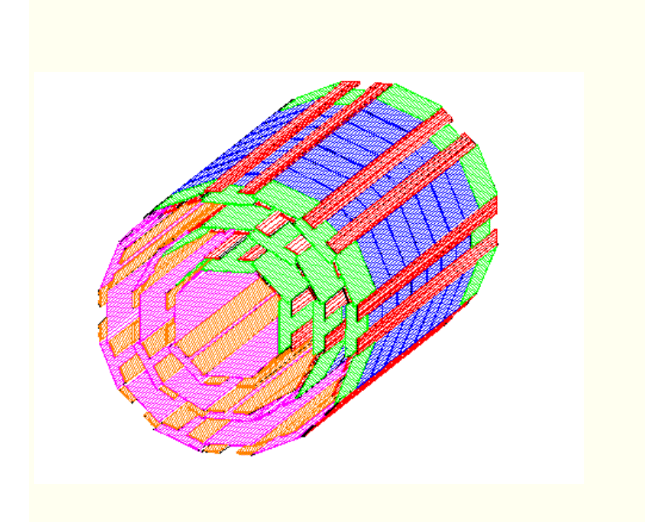
\includegraphics[width=7cm]{STAR_Detectors/SVD_3_Layers} }}%
    \qquad
    \subfloat[\centering Φωτογραφία του SVT            ]{{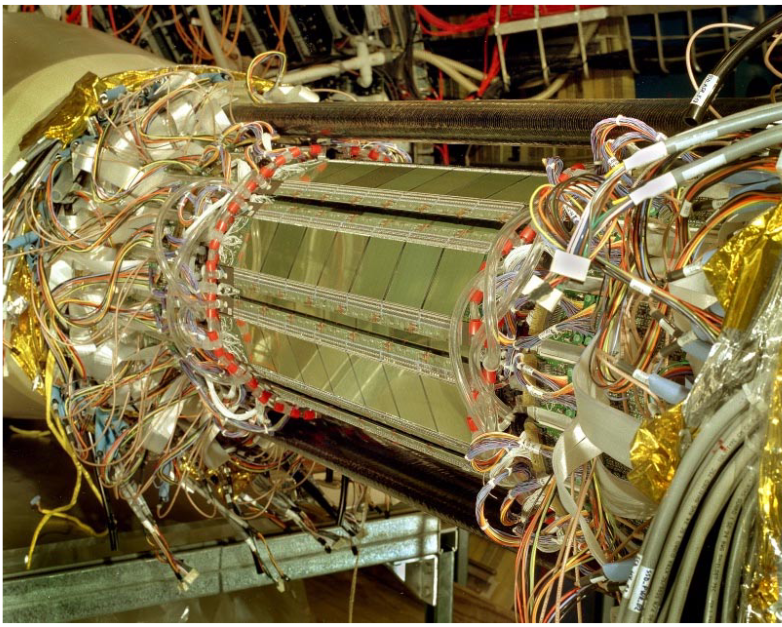
\includegraphics[width=7cm]{STAR_Detectors/SVD_photo} }}
    \caption{Η δομή του SVT}%
    \label{fig3.13}%
\end{figure}	
	
	
	Ο SVT αποτελείται από τρία στώματα Silicon Drift Detectors (SDD). Το κάθε στρώμα αποτλείται από 8,12,16 ράβδους στήριξης οι οποίες τοποθετούνται περιμετρικά της δέσμης και η κάθε ράβδος συγκρατεί 4, 6, 7 τμήματα SDD αντίστοιχα σε κάθε στρώμα, άρα συνολικά υπάρχουν 216 τμήματα SDD. Τα στρώματα είναι σε ακτίνες 5.9cm, 10.2cm, 14.9cm από την δέσμη και το συνολικό μήκος είναι 44.1cm. Ο μεγάλος αριθμός από ανιχνευτικά τμήματα σε τόσο μικρό χώρο είναι αναγκαίος διότι εκεί θα υπάρχουν οι μεγαλύτερες συγκεντώσεις φορτισμένων σωματιδίων, περιπου 1500-3000 ανά γεγονός. 
	
	Ας δούμε τώρα τι ακριβώς είναι οι SDD. Θα μπορούσαμε να τους φανταστούμε ως  κάτι σαν Time Projection Chambers αλλά στερεάς κατάστασης. Ο πιό απλός τέτοιου τύπου ανιχνευτής στερεάς κατάστασης θα αποτελούταν από μία επίπεδη επαφή p-n από Si. Αν φέρουμε σε επαφή έναν ημιαγωγό τύπου p και έναν n, τότε οι οπές του p και τα ηλεκτρόνια του n κινούνται λόγω διάχυσης προς αντίθετες κατευθύνσεις, γεννώντας ένα ρεύμα διάχυσης $I_0$. Κατά την κίνησή τους επανασυνδέονται και δημιουργείται μία περιοχή απογύμνωσης. 
	Αυτή η περιοχή, δεδομένου ότι από τον n έχουν απομακρυνθεί κάποια ηλεκτρόνια, γίνεται θετικά φορτισμένη με οπές από την μερία του n και αντίστοιχα αρνητικά φορτισμένη με ηλεκτρόνια από την μεριά του p. Έτσι, δημιουργείται και ένα ηλεκτρικό πεδίο από την n στην p. Αυτό το πεδίο αντιστέκεται στην διάχυση των φορέων και εν τέλει επιτυγχάνεται μία κατάσταση ισορροπίας στην οποία μηδενίζεται το ρεύμα.
	
	 Εφαρμόζοντας τώρα διαφορά δυναμικού μεταβάλλουμε το πλάτος της περιοχής απογύμνωσης, το ηλεκτρικό πεδίο εντός αυτής και κατ' επέκταση το ρεύμα θα δίνεται από την σχέση 
	 \begin{align}\label{eq3.6}
	 	I = I_0 (exp(\frac{qV}{kT})-1) 
	 \end{align}
%	και η αντίστοιχη αντίσταση που δημιουργείται από την 
%	\begin{align}\label{eq3.7}
%		R_F = \left( \odv{I}{V}\right)^{-1} = \frac{kT}{qI}
%	\end{align}
	Όπως έχει ήδη αναφερθεί, στην κατάσταση ισορροπίας και χωρίς εξωτερική τάση, V=0, το ρεύμα μηδενίζεται. Αν εφαρμόσουμε ορθή πόλωση ($V>0$) δηλαδή μεγαλύτερο δυναμικό στην p περιοχή, μικραίνουμε το μήκος της περιοχής απογύμνωσης και τότε ηλεκτρόνια και οπές χρειάζονται μικρότερη ενέργεια για να μεταπηδήσουν το φράγμα δυναμικού και να πάνε στην άλλη περιοχή άρα το ρεύμα αυξάνεται. Αυτό υποδεικνύει και η εξίσωση (\ref{eq3.6}). 
	Αντιθέτως, αν εφαρμόσουμε ανάστροφη πόλωση, $V<0$, τότε το ρεύμα μειώνεται και η περιοχή απογύμνωσης μεγαλώνει καθώς τα αρνητικά φορτία του n ημιαγωγού κατευθύνονται στην περιοχή θετικής τάσης που εφαρμόζεται στην άκρη του και αντίστοιχα οι θετικές οπές του p κατευθύνονται προς την περιοχή αρνητικής τάσης που εφαρμόζεται στην άκρη του.
	
	Εμείς θέλουμε να εκμεταλλευτούμε τις ιδιότητες μίας επαφής p-n προκειμένου να κατασκευάσουμε έναν ανιχνευτή. Η ιδέα είναι ότι όταν ένα φωτόνιο ή ένα φορτισμένο σωματίδιο εισέλθει στην περιοχή απογύμνωσης, ενδέχεται να αλληληπιδράσει με τον Si και να δημιουργήσει εξτρα ζεύγος ηλεκτρονίου-οπής τα οποία θα οδηγηθούν σε αντίθετες κατευθύνσεις εξαιτίας του πεδίου και θα συλλεχθούν στα άκρα των περιοχών p, n από ηλεκτρόδια. Συγκεκριμένα, ένα φωτόνιο θα δημιουργήσει μόνο ένα ζεύγος, ενώ ένα φορτισμένο σωματίδιο αναμένουμε να δημιουργήσει ζεύγη κατά μήκος της τροχιάς.
	 
	 Εμείς θέλουμε να κατασκευάσουμε μία κατάσταση στην οποία το ρεύμα λόγω διάχυσης θα είναι μικρό σε σύγκριση με το ρεύμα που δημιουργείται από τις αλληλεπιδράσεις, επομένως αυτά να μπορούν να διαχωριστούν. Άρα θα χρησιμοποιήσουμε ανάστροφη πόλωση. Η ανάστροφη πόλωση μεγαλώνει την περιοχή απογύμνωσης, δηλαδή την περιοχή στην οποία θα γίνουν οι αλληλεπιδράσεις με τα σωματίδια που θέλουμε να ανιχνεύσουμε.
	Όταν αυξήσουμε αρκετά την διαφορά δυναμικού, τότε φτάνει σε μία τιμή $V_D$, στην οποία η απογύμνωση είναι πλήρης και όλοι οι φορείς έχουν απομακρυνθεί στις διόδους αφήνοντάς την ουδέτερα φορτισμένη.	
	%
	Μία τέτοια δίοδος που  έχει φορείς υψηλής κινητικότητας και μικρό όγκο,  είναι κατάλληλη για να τοποθετηθεί ως ανιχνευτής σε περιοχές υψηλής ροής σωματιδίων, όπως εκεί που τοποθετείται στο STAR.
	
	Η ιδέα συγκεκριμένα για τους SDD πηγάζει από την απλή δίοδο όπως αυτή που περιγράφηκε φτιαγμένη από Si. 
	Γενικά, δεν φέρνουμε ακριβώς σε επαφή τους n \& p ημιαγωγούς αλλά παρεμβάλλουμε μεταξύ τους κάποιον άλλον ημιαγωγό, με πολύ χαμηλότερη συγκέντρωση προσμίξεων, στην περιοχή του οποίου δημιουργούνται τα ζεύγη ηλεκτρονίων-οπών από τα σωματίδια. 
	Η πιό απλή περίπτωση είναι να έχουμε έναν κύριο όγκο από τέτοιο υλικό και κατά μήκος δύο απέναντι πλευρών του να τοποθετήσουμε την άνοδο (n ημιαγωγός) και την κάθοδο (p ημιαγωγός) όπου θα μαζεύονται τα ζεύγη ηλεκτρονίων-οπών που θα δημιουργούν τα προς ανίχνευση σωματίδια.
	Ωστόσο, αυτό μπορεί να λειτουργήσει ακόμη και όταν οι παραπάνω ημιαγωγοί δεν καλύπτουν πλήρως τα άκρα της διόδου όπως φαίνεται στην Εικόνα (\ref{fig3.14}a).
	Τότε δημιουργείται επιπλέον χώρος και μπορούμε  πάρουμε τον n από την μία πλευρά του κύριου όγκου και να τον τοποθετήσουμε δίπλα από τον p, χωρίς βέβαια να ακουμπάνε (Εικόνα (\ref{fig3.14}b). Έτσι αφήνουμ χώρο για έναν ακόμη p ημιαγωγό στην κάτω πλευρά του Si. 
	Τότε, σε χαμηλές τάσεις δημιουργούνται δύο φορτισμένες περιοχές γύρω από τους p εντός του Si oι οποίες διαχωρίζονται από μία ουδέτερη ζώνη (Εικόνα \ref{fig3.15}c). Για μεγαλύτερη διαφορά δυναμικού το πλάτος της ουδέτερης περιοχής μειώνεται και συγκεντρώνεται γύρω από τον n ημιαγωγό, ενώ οι δύο φορτισμένες περιοχές θα έχουν κοινό όριο και στο εσωτερικό τους θα υπάρχουν αντίθετα πεδία που κατευθύνονται προς τους ημιαγωγούς p (Εικόνα (\ref{fig3.14}d).
	Δημιουργείται έτσι μία περιοχή στην οποία τα ηλεκτρόνια έλκονται μόνο από την άνοδο, τον ημιαγωγό n και οι αντίστοιχες οπές κατευθύνονται ταχύτατα προς τις καθόδους, τους ημιαγωγούς p.
	Αν τώρα τοποθετήσουμε επιπλέον ηλεκτρόδια μπορούμε να βελτιώσουμε την ολίσθηση ηλεκτρονίων και οπών εντός του κύριου ημιαγώγιμου υλικού προς τα ηλεκτρόδια (Εικόνα (\ref{fig3.15})).
	%Δημιουργείται έτσι ένα πλατώ δυναμικού για τα ηλεκτρόνια στο οποίο κινούνται μόνο με διάχυση εως ότου φτάσουν στην περιοχή όπου θα έλκονται από την άνοδο. 
	%Ακόμη, για να βοηθηθεί η κίνηση των ηλεκτρονίων προς την άνοδο, τοποθετούμε επιπλέον εξωτερικό ηλεκτρικό πεδίο. 
%	\begin{figure}[h!]
%		\centering 
%		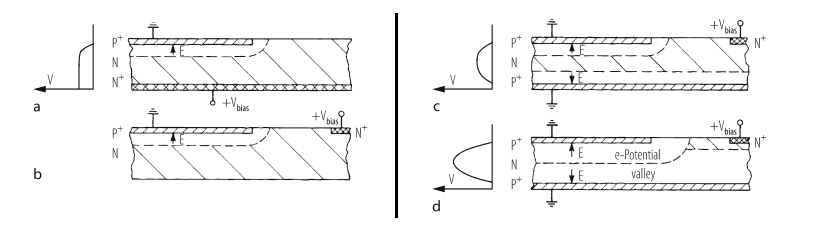
\includegraphics[scale=0.7]{STAR_Detectors/SDD}
%		\caption{Η ιδέα πίσω από τους SDD}
%		\label{fig3.14}
%	\end{figure}	
	\begin{figure}[h!]
    \centering
    \begin{minipage}{.5\textwidth}
        \centering
        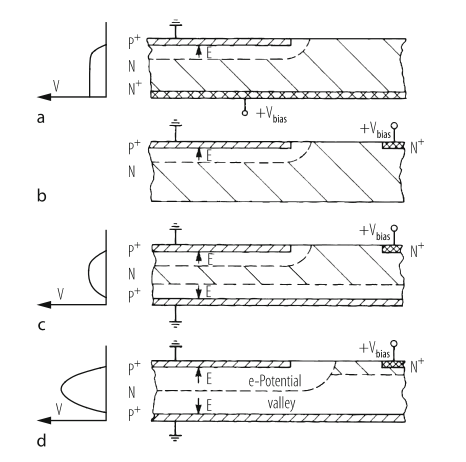
\includegraphics[scale=0.6]{STAR_Detectors/SDD_v}
        \caption{Αρχή Λειτουργίας ενός SDD}
        \label{fig3.14}
    \end{minipage}%
    \begin{minipage}{0.5\textwidth}
        \centering
        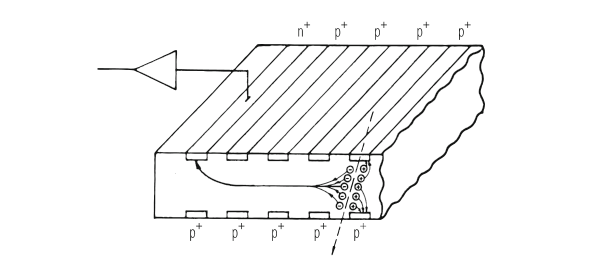
\includegraphics[scale=0.7]{STAR_Detectors/SDD_2}
        \caption{Τελικός SDD με όλες τις ανόδους/καθόδους}
        \label{fig3.15}
    \end{minipage}
\end{figure}
	
	Ο κάθε SDD του STAR έχει πάχος 280μm και καλύπτει μία επιφάνεια 63mm$\times$63mm. Οι άνοδοι τοποθετούνται σε βάθος 250μm και έχουν διαστάσεις 200μm$\times$200μm οι οποίες είναι βολικές για την καταγραφή σημάτων από ηλεκτρόνια των οποίων η διάχυση εντός του Si διαρκεί $\sim \mu sec$ και αποκτά πλάτος $\sim 100\mu m$ σε συνολική απόσταση $\sim 3cm$. 

	%Ένα σημαντικό σημείο είναι να επιτευγχθεί η βέλιτιστη διακριτική ικανότητα στην διεύθυνση ολίσθησης. Για κάτι τέτοιο απαιτείται η ταχύτηα ολίσθησης των παραγόμενων ηλεκτρονίων να είναι γραμμική προς το πεδίο $u_{dr} = \mu_e E$. Ακόμη, θα πρέπει να είναι  γνωστή η λειτουργία των ανιχνευτών 
	%με μεγάλη ακρίβεια η θέση των ανιχνευτών. Συνεπώς, πρωτού την κανονική τους λειτουργία γίνεται η χαρτογράφησή τους κάτω από παρόμοιες συνθήκες. Έτσι, όταν πραγματοποιούνται τα πειράματα μπορούν να 
		
	Η άνοδος στην οποία παράγεται το εκάστοτε σήμα από ηλεκτρόνια, καθώς και ο χρόνος ολίσθησης καθορίζουν τις συντεταγμένες της τροχιάς, ενώ ταυτόχρονα μετρήσεις της απώλειας ενέργειας $dE/dx$, δίνουν ταυτοποιήση των σωματιδίων (Εικόνα (\ref{fig3.1}) 
	
	\begin{figure}[h!]
		\centering 
		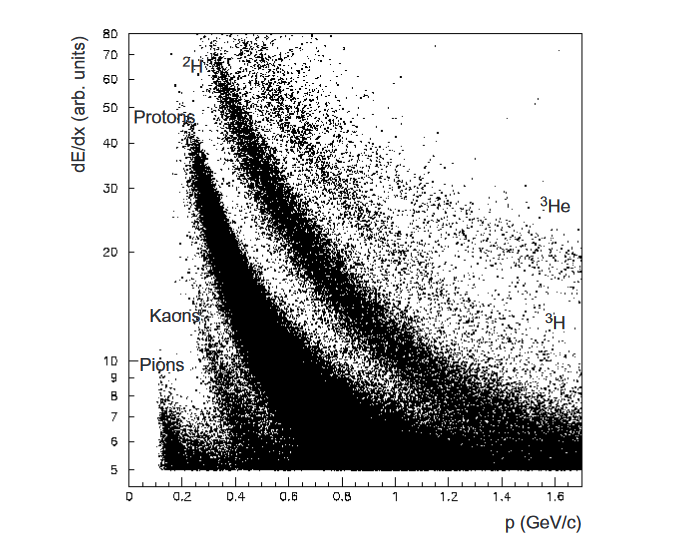
\includegraphics[scale=0.5]{STAR_Detectors/SDD_dedx}
		\caption{Μετρήσεις απώλειας ενέργειας dE/dx σε συγκρούσεις Au-Au 11.6GeV/n στο AGS}
		\label{fig3.}
	\end{figure}
	
	
	